\chapter{I Was on Food Stamps... Now I Make \$100M/Year}

In this School of Hard Knocks interview, curated by LazyingArt LLC through Video2Book, the episode proceeds almost like a proof stated backward. We are shown the end first --- mansion, cars, scale, food-stamps origin, bankruptcy without a broke mindset --- and only afterward are we led through the mechanisms that are supposed to make those results intelligible: the refusal to sell hours forever, the purchase of existing playbooks, the arithmetic of cash flow, the practical force of belief, and the business necessity of visibility.

\section{Cold Open: Scale Before Explanation}

The episode opens with a teaser splice rather than a settled beginning. Before the interview is properly introduced, we are given the endpoint in fragments: a year somewhere near one hundred million dollars across companies, a personal figure in the eight figures, the memory of government cheese and food stamps, the claim that everything could be rebuilt, the preference for buying businesses over building blindly, and a brief turn toward faith. The structure matters. We are meant to see the conclusion before we are told the premises.

The first pair of financial markers are separated almost immediately. One figure belongs to company scale, the other to the speaker personally:
\begin{align}
R_{\text{companies,max}} &\approx \$90\text{--}100\,\text{million}, \\
Y_{\text{personal}} &\approx \$25\,\text{million}.
\end{align}
The chapter should keep these categories distinct from the start. The transcript is careful enough, even in conversation, to separate revenue across companies from what the speaker says he made for himself.

\begin{figure}[h]
\centering

\includegraphics[width=0.78\textwidth]{lecture_53_figure_02.png}
\caption{TJ's personal one-year money claim, visually preserved in the interview itself.}
\end{figure}

Near this moment we can cleanly reconstruct the visible numerical claim as
\begin{equation}
Y_{\text{personal}} \approx \$25\,\text{million}.
\end{equation}
The image itself shows only the number, not an accounting category, so we keep the notation cautious.

After the teaser, the host resets the scene and frames the episode as a Beverly Hills business masterclass. These host-side markers are part of the lecture's scale-setting apparatus:
\begin{align}
V_{\text{house}} &\approx \$50\,\text{million}, \\
N_{\text{companies}} &\approx 10, \\
R_{\text{portfolio,current}} &> \$100\,\text{million}/\text{year}.
\end{align}
These are framing quantities. They help explain why the host thinks this is the right person to ask, but they should not be fused with the speaker's own more specific statements.

\section{Origin, Scale, and the Refusal of a Broke Mindset}

Once the interview begins in earnest, the lecture stabilizes. The host first establishes that the speaker has been a business owner for most of his life. We are told of a tech-services business built and sold, then a construction business built and sold, and a supplement business in the present. This gives the later advice some weight; it is not being delivered from one lucky exit alone, but from repeated operating experience.

Only then does the lecture pivot backward into biography. No rich parents appear in this story. Instead we are given an early pregnancy, the American South, food stamps, government cheese, and the desire to get out. The important move is that poverty is not treated here as a total description of the self. The decisive statement is conceptual before it is motivational:
\begin{equation}
\text{no money} \neq \text{broke mindset}.
\end{equation}
This distinction governs much of the interview. It is what later allows the speaker to say both that he has been broke and that he was never broke in the deeper sense he cares about.

\subsection{Question \& Answer}

\paragraph{Question.} What is the real difference between having no money and having a broke mindset?

\paragraph{Answer.} In the lecture, having no money is a condition. A broke mindset is an internal ceiling. One can endure the first and refuse the second. That is why the speaker can place food stamps, hardship, and even bankruptcy inside the same story without surrendering the claim that he was always thinking beyond where he stood. The chapter should preserve this distinction because later claims about rebuilding, risk, and acquisition all depend on it.

The lecture then makes a further refinement. The childhood desire was not initially phrased as a precise wish to build a hundred-million-dollar company. It was more primitive and perhaps more powerful: to get out and never come back. The money target arrives later; the directional pressure comes first.

\section{From Hours to Systems}

The next major movement is not a biography beat but a doctrine beat. Asked about financial advice, the speaker does not offer a market prediction. Instead he gives a structural warning: do not trade dollars for hours forever. Whatever the hourly rate may be, the model is bounded by time itself. A compact reconstruction of the lecture's logic is
\begin{equation}
Y_{\text{labor}} \le r_h H,
\end{equation}
where \(r_h\) is the hourly rate and \(H\) is the number of hours one can sell. If income is tied only to presence, then even a generous rate remains trapped inside the finite quantity \(H\).

The counter-rule is equally simple:
\begin{equation}
Y_{\text{sleep}} > 0.
\end{equation}
This is not mystical notation. It is the lecture's shorthand for systems, assets, investments, or businesses that continue producing while one is not actively trading time.

\subsection{Question \& Answer}

\paragraph{Question.} How do we stop trading time for money?

\paragraph{Answer.} The lecture's answer is not that labor is contemptible. It is that labor by itself is not enough. We begin with work, but we should try to convert work into a system that remains productive when we are absent. In the interview this appears under several names --- passive income, building systems, investing, making money in one's sleep --- but the mechanism is the same. We move from \(Y_{\text{labor}}\) toward \(Y_{\text{sleep}}\).

This transition also explains why the next question arrives when it does. Once we accept that hours alone are insufficient, we must ask what concrete path is open now, not in theory but in today's market.

\section{Buy the Playbook}

When the host asks what someone should do now, the answer first allows real estate as a respectable route. But the lecture does not stop there. It pivots quickly to the more distinctive thesis: if one were starting today, one should buy businesses. The force of the claim lies in a single phrase repeated by the speaker: the playbook is already there.

We can compress the lecture's thought as
\begin{equation}
\text{existing business} \to \text{existing playbook} \to \text{faster path than starting from zero}.
\end{equation}
This is a rejection of the romantic assumption that entrepreneurship must always begin with the blank page. In the episode, the stronger move is to purchase an already-working system and step into visible demand.

\subsection{Question \& Answer}

\paragraph{Question.} Why buy a business instead of building one from scratch?

\paragraph{Answer.} Because the lecture treats a working business as condensed knowledge. Customers, processes, pricing, operating rhythm, and proof of demand are already present. One is not forced to invent every line of the playbook. The argument is therefore not merely about speed for its own sake; it is about stepping into a machine whose existence has already answered several of the hardest questions.

The speaker then makes the claim more mechanical. He mentions SBA \(7\)A financing and other forms of creative financing, then turns to cash-flowing businesses such as laundromats, pool companies, and vending machines. The emphasis is not prestige but regularity. We are pushed toward assets that are not overly labor-intensive and that survive downturns reasonably well.

\paragraph{Worked Example.} The interview gives a simple monthly spread example. We keep it with a small caveat: the spoken arithmetic is approximate, so the cleaned form below should be read as an illustrative ledger rather than a literal audit.
\begin{align}
CF_{\text{business}} &\approx \$20{,}000/\text{month}, \\
DS &\approx \$7{,}000\text{--}\$10{,}000/\text{month}, \\
S &= CF_{\text{business}} - DS.
\end{align}
If we take the lecture at the point of its intended conclusion, then the retained spread is roughly
\begin{equation}
S \approx \$10{,}000/\text{month}.
\end{equation}

We may state the logic of the example in short steps:
\begin{enumerate}
\item Find a business whose monthly cash flow is already visible.
\item Finance the acquisition through SBA \(7\)A or other creative means.
\item Service the debt from the business's own operating cash flow.
\item Retain the spread \(S\) as the immediate economic upside.
\end{enumerate}

\begin{figure}[h]
\centering
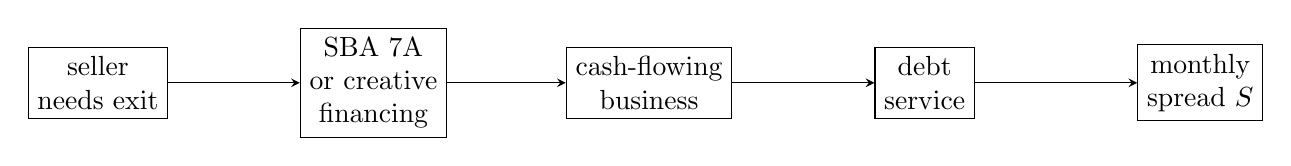
\begin{tikzpicture}[>=stealth]
\node[draw, rectangle, align=center] (a) at (0,0) {seller\\needs exit};
\node[draw, rectangle, align=center] (b) at (3.5,0) {SBA \(7\)A\\or creative\\financing};
\node[draw, rectangle, align=center] (c) at (7.0,0) {cash-flowing\\business};
\node[draw, rectangle, align=center] (d) at (10.5,0) {debt\\service};
\node[draw, rectangle, align=center] (e) at (14.0,0) {monthly\\spread \(S\)};

\draw[->] (a) -- (b);
\draw[->] (b) -- (c);
\draw[->] (c) -- (d);
\draw[->] (d) -- (e);
\end{tikzpicture}
\caption{Transcript-backed reconstruction of the acquisition logic: exit pressure, financing, cash flow, debt service, and retained spread.}
\end{figure}

\section{Seller Pressure and the Gray Tsunami}

The next question is exactly the right one: where do we find these businesses? The lecture answers by descending from doctrine to search. One may use listing portals, business brokers, or simple cold calls. The most important point is that some owners would sell if asked, even if they are not yet formally in motion.

Then the frame widens from search technique to demographic structure. The host names a large transfer of wealth; the speaker answers with the term ``gray tsunami.'' The content of that term is that many boomer owners need to exit, while many children do not wish to inherit the family operation. In a compressed inequality,
\begin{equation}
N_{\text{sellers}} > N_{\text{buyers}}.
\end{equation}
This should not be mistaken for a measured census claim inside the interview. It is a directional model. Its purpose is to say that the speaker's acquisition advice is not floating free in the air; it is attached to a specific historical moment in which supply of aging-owner exits may exceed the number of prepared buyers.

This is why the lecture's business-buying thesis has more than one premise. It requires a playbook, financing, cash flow, and demographic timing. Remove any one of these, and the recommendation becomes thinner than the speaker intends.

\section{Faith as a Practical Variable}

A brief community interlude interrupts the conversation, but even this interruption continues one of the lecture's main motifs: the need for blueprint, access, and proximity to operators. When the interview returns, however, the register changes. The speaker is asked whether he believes in God, and a childhood story follows: a poor environment, tears, doubt, a plea for revelation, and then an encounter at work that becomes decisive.

The lecture could have left this in the register of autobiography. It does not. Instead it turns faith into a practical variable:
\begin{equation}
\text{belief} \to \text{actions},\ \text{thought},\ \text{relationships}.
\end{equation}
This is the business use of the story. Belief is treated not merely as a spiritual confession but as something that governs conduct and therefore affects opportunity.

\subsection{Question \& Answer}

\paragraph{Question.} Why does faith matter practically in business rather than only spiritually?

\paragraph{Answer.} Because in the lecture belief is causal. If we truly believe something, then we act under that belief, think through that belief, and build relationships under that belief. The point is not to convert theology into finance. The point is to show that deep conviction shapes economic behavior long before any spreadsheet appears.

The lecture then narrows again. Asked about college, the speaker does not say it was useless. He says it gave him a skill set, specifically programming, and helped him become a computer programmer. What it did not do, by itself, was make him a millionaire. This distinction prepares the next topic: what formal business education misses.

\section{Skill, Marketing, and the Expansion of the Possible}

From college the lecture moves directly to business school and then to marketing. The answer is sharp: what school does not teach well enough is that people may need what one has, but they do not know who one is. The problem is often not intrinsic value but obscurity. We can state the lecture's claim as
\begin{equation}
\text{people need you} \land \neg(\text{they know you}) \to \text{marketing problem}.
\end{equation}
And its positive counterpart is
\begin{equation}
\text{need} \to \text{visibility} \to \text{growth}.
\end{equation}
The speaker's vivid phrasing about climbing the highest mountain and telling people who you are amounts to a theory of exposure, not a theory of product invention. One may have the sauce and still fail if the market cannot see it.

\subsection{Question \& Answer}

\paragraph{Question.} What does business school fail to teach once the product or skill already exists?

\paragraph{Answer.} In the lecture, the missing piece is marketing. Business knowledge may tell us how a firm works in principle, but growth requires that the right people know we exist. The bottleneck is therefore often not internal competence but external visibility.

The final movement of the interview uses place as argument. The speaker walks through Beverly Park, points out celebrity compounds, massive garages, and neighborhoods of extreme scale, and then states the real lesson: once we see certain levels of possibility, we cannot entirely unsee them. The chapter can carry that in compact form as
\begin{equation}
\text{see larger ceiling} \to \text{cannot unsee possibility}.
\end{equation}
This environmental shift then feeds the closing worldview. Wealthy people, in the speaker's account, do not live primarily inside a predetermined ladder of raises and positions. They look for problems to solve and solutions to create:
\begin{equation}
\text{problem} \to \text{solution} \to \text{money}.
\end{equation}
The line about wealthy people not needing structure should be read carefully. It does not mean the wealthy never build systems. It means they are less likely to accept externally imposed ceilings as the only available structure.

\section{Summary}

The lecture begins with spectacle and ends with a theory. Its order matters. First it shows scale, then it separates company revenue from personal income, then it moves backward to poverty and mindset, then forward to the refusal to sell hours forever, then further into acquisition arithmetic, seller pressure, and historical timing. Only after those mechanisms are in place does it widen to faith, skill, marketing, and environment.

What remains after the episode is not one isolated slogan but a connected chain. We are asked to distinguish condition from mindset, hours from systems, blank-page invention from existing playbooks, sellers from buyers, belief from mere ornament, and usefulness from visibility. The lecture's strongest claim is that wealth is not only a number at the end. It is a sequence of conceptual separations that, once seen clearly enough, begin to change what action becomes thinkable.